\documentclass[11pt,a4paper]{article}

\usepackage[margin=2.5cm]{geometry}
\usepackage{booktabs}
\usepackage{graphicx}
\usepackage{amsmath}
\usepackage{xcolor}
\usepackage{caption}
\usepackage{float}
\usepackage[hidelinks]{hyperref}
\usepackage{enumitem}

\definecolor{deepblue}{RGB}{31,78,99}
\definecolor{midblue}{RGB}{46,139,168}

\newcommand{\cat}[1]{\texttt{#1}}
\newcommand{\found}[0]{\textcolor{deepblue}{\textbf{found}}}
\newcommand{\missed}[0]{\textcolor{red!70!black}{\textbf{missed}}}
\newcommand{\unreach}[0]{\textcolor{gray}{\textbf{unreachable}}}

\title{\textbf{Do Simulated Conversations Reproduce Real Agent Failures?}\\
\large A Scorer-Parity Comparison and Scale Study of the TechRepair WhatsApp Support Agent}
\author{Eduardo Fernandez Salazar\\
\small Imperial College London \;\textperiodcentered\; MSc Artificial Intelligence \;\textperiodcentered\; Pulpoo / TechRepair Polanco}
\date{24 July 2026}

\begin{document}
\maketitle

\begin{abstract}
\noindent
Synthetic adversarial testing of conversational agents is widely used, but whether the failures
it produces correspond to the failures that occur in real production is rarely measured. We compare
1{,}299 real Spanish WhatsApp support conversations from a deployed TechRepair service agent
(376 failures under a rule-based, LLM-free scorer) against up to 2{,}560 simulated conversations
generated by LLM personas talking to a \emph{verbatim} copy of the same production agent running
on a fully seeded fake database. Both corpora are labelled by the \emph{identical} scorer and
projected onto a frozen 16-category failure taxonomy, giving scorer parity by construction.
The simulation reproduces 5 of 7 reachable real failure categories (71\%), including the dominant
production failure mode (loops/stalls: 68\% of real failures, 81\% of simulated), at a similar
overall failure rate (21\% vs 29\%). A seven-batch scale study ($N=10$ to $N=1000$) shows category
coverage saturates at $N\!\approx\!50$ and never improves thereafter: the two absent categories
(comprehension, data-gap failures --- jointly present in over half of real failures) are
\emph{structurally} unreachable under current user simulators and test-data seeding, not
budget-limited. The Jensen--Shannon divergence between real and simulated failure distributions is
scale-invariant at $\approx 0.24$ bits (sampling noise floor: $0.005$), demonstrating that
increasing simulation volume buys statistical precision and failure volume, but not new failure
kinds. We conclude that simulation power is gated by simulator design --- persona realism and
backend-data imperfection --- rather than by scale, and quantify exactly which production failure
modes remain out of reach.
\end{abstract}

\section{Introduction}

Conversational agents deployed to customers fail in ways their test suites did not anticipate.
The dissertation this report belongs to (\emph{Closing the Loop Between Synthetic Agent Testing
and Production Reality}) asks whether synthetic testing predicts production failures. Earlier
\emph{static-mode} analysis answered a design-level version of that question: test suites
generated without production knowledge \emph{target} only a small fraction of observed production
failure categories (recall $0.068$). This report answers the stronger, behavioural version:

\begin{quote}
\itshape When simulated users converse with the real agent code, do the failures that actually
emerge match the failures observed in production --- in kind, in frequency, and in mechanism?
And how does that correspondence grow with the number of simulations?
\end{quote}

\noindent This became answerable when the production agent was reproduced \emph{verbatim} inside
a controlled simulation: identical prompts, LangGraph structure, and guardrails, with only the
database layer replaced by a fully specified in-memory fake. The agent cannot distinguish the
simulation from production; its only live dependency is its own LLM calls.

\paragraph{Contributions.}
\begin{enumerate}[itemsep=2pt]
  \item A \textbf{scorer-parity methodology}: both corpora are labelled by the same rule-based,
        LLM-free failure scorer and projected onto a frozen shared taxonomy, eliminating
        judge-model bias from the comparison itself (\S\ref{sec:method}).
  \item A \textbf{correspondence result}: 5/7 reachable real failure categories reproduced,
        with the production-dominant loop/stall mode reproduced as the simulation-dominant mode
        (\S\ref{sec:results}).
  \item A \textbf{scale study} across seven independent batches ($N=10\ldots1000$; 2{,}560
        conversations) showing coverage saturation at $N\!\approx\!50$ and scale-invariant
        distributional divergence (\S\ref{sec:scale}).
  \item A \textbf{reachability analysis} separating structurally unreachable failure modes from
        budget-limited ones, with the mechanisms identified (\S\ref{sec:discussion}).
\end{enumerate}

\section{Data}
\label{sec:data}

\subsection{Real corpus}
The production corpus contains \textbf{1{,}299 conversations} (24{,}537 messages) between real
customers and the deployed TechRepair WhatsApp support agent, exported once and anonymised by a
three-pass pipeline (regex, Spanish NER, brand scrub); all experiments run offline on the
anonymised corpus. Structured operational signals accompany each conversation: escalation records,
human takeovers, message delivery statuses, intent/confidence telemetry, and timestamps
(291 escalations; 22.4\%).

\subsection{Simulated corpora}
The simulation target is the production agent copied verbatim into a sandbox
(\texttt{tech_repair-live-agent/}): byte-identical prompts, the same graph and guardrails, an
in-memory Supabase-compatible fake database seeded with one fully specified fictitious customer
(two service orders exercising both warranty states, a disclosure-gated order, CRM memory, and
escalation rules). Simulated users are LLM personas (Claude Haiku, Spanish) generated by the
platform's Phase~B pipeline from the agent's own structure (MAP-Elites persona library,
scenario catalogue with adversarial variants), equipped with the fake customer's identifying
context. Conversations run over HTTP with per-test session isolation and per-batch database
resets. The primary corpus for the distribution comparison pools 390 conversations from three
independent runs; the scale study adds 2{,}560 more in seven independent batches.

\section{Methodology}
\label{sec:method}

\subsection{Scorer parity}
The methodological core is that \emph{the same} failure detector labels both corpora.
The production scorer is rule-based and LLM-free: it reads only operational signals ---
escalations, explicit human requests (Spanish pattern lexicon), message counts, verbatim customer
repetition, verbatim agent repetition, delivery failures, expiry without resolution, frustration
lexicon, and customer pushback wording. It emits a weighted failure score and one or more of eight
production failure categories. A conversation is a failure when its score is $\geq 3$ \emph{and}
at least one category triggered --- the same ground-truth criterion used for the real corpus
(376/1{,}299 failures).

Simulated conversations are adapted to the production message schema by a thin, faithful mapping
(user$\to$customer, agent$\to$ai\_agent, tool calls preserved, persona abandonment $\to$ expiry,
filed escalations $\to$ escalation records). Telemetry that does not exist in simulation
(intent detection, confidence scores, delivery statuses) is left absent, exactly as it would be
for a production conversation missing those fields. No signal is invented for either side.

\subsection{Shared taxonomy and projection}
Both category vocabularies project onto a frozen 16-category shared
taxonomy\footnote{Version \texttt{1.0-frozen-2026-07-14}; frozen mid-campaign so that
precision/recall comparisons stay meaningful against a fixed vocabulary.} through total,
import-time-checked mappings.
All distributional comparisons are expressed in that taxonomy.

\subsection{Distributional comparison}
Let $P$ and $Q$ be the normalised distributions of category labels among failed conversations in
the real and simulated corpora, over the pre-registered \emph{reachable support} (\S\ref{sec:reach}).
We report the Jensen--Shannon divergence
\begin{equation}
\mathrm{JSD}(P\,\|\,Q) \;=\; \tfrac{1}{2}\,D_{\mathrm{KL}}\!\left(P \,\middle\|\, M\right)
                        \;+\; \tfrac{1}{2}\,D_{\mathrm{KL}}\!\left(Q \,\middle\|\, M\right),
\qquad M = \tfrac{1}{2}(P+Q),
\end{equation}
in bits (symmetric, bounded $[0,1]$), with 95\% bootstrap confidence intervals (1{,}000
conversation-level resamples). Two anchors make the number interpretable: a \textbf{noise floor}
(mean JSD between random halves of the real corpus itself, $0.0050$; p95 $0.0108$) and the
\textbf{real-vs-uniform} JSD ($0.2014$). Per-category rates carry Wilson 95\% intervals.

\subsection{Reachability pre-registration}
\label{sec:reach}
Before running, each production category was classified by whether the simulator \emph{could}
produce it: \cat{delivery\_infra} is \emph{unreachable} (no WhatsApp transport layer exists in
simulation); \cat{comprehension} is \emph{partial} (the customer-repetition signal exists, but
intent/confidence telemetry does not); \cat{data\_gap} is \emph{partial} (a single fully seeded
customer leaves little room for missing backend data); the remaining five are fully reachable.
Two failure-mode predictions were pre-registered from the literature: simulated users are
systematically over-cooperative and rarely repeat themselves verbatim or express frustration
(Lost in Simulation; Synthetic Users, Real Differences), and a complete test database suppresses
data-gap failures.

\subsection{Scale study design}
\label{sec:scaledesign}
Seven \textbf{independent} batches of $N\in\{10,50,100,200,400,800,1000\}$ conversations were
executed sequentially against the live agent (six workers; fresh database reset per batch;
deterministic seeded suites: for $N\leq150$ a seeded sample of the 150-test suite, above that the
full suite plus seeded resampled duplicates with fresh test identities). Per batch we measure
failure count and rate, distinct categories found, coverage of reachable real categories, JSD to
the real distribution, wall time, and persona cost; the same metrics are computed cumulatively
over the pooled batches (2{,}560 conversations).

\section{Results: correspondence at fixed scale}
\label{sec:results}

\subsection{Corpus-level rates}
Under the identical scorer and threshold, the two corpora fail at similar rates
(Table~\ref{tab:corpus}): 28.9\% of real conversations versus 21.0\% of simulated ones.

\begin{table}[H]
\centering
\caption{Corpus-level failure rates under the identical rule-based scorer (min score $=3$).}
\label{tab:corpus}
\begin{tabular}{lrrr}
\toprule
 & Conversations & Failures & Failure rate \\
\midrule
Real (production)        & 1{,}299 & 376 & 28.9\% \\
Simulated (pooled runs)  &   390   &  82 & 21.0\% \\
\bottomrule
\end{tabular}
\end{table}

\subsection{Reachability matrix}
Table~\ref{tab:reach} is the study's central artefact: for each production category, whether the
simulator could produce it, and whether it did.

\begin{table}[H]
\centering
\caption{Reachability matrix (production vocabulary; counts are failures carrying each label).}
\label{tab:reach}
\begin{tabular}{llrrl}
\toprule
Production category & Reachability & Real & Sim & Status \\
\midrule
\cat{comprehension}       & partial     & 153 &  0 & \missed \\
\cat{resolution}          & reachable   & 221 & 22 & \found  \\
\cat{data\_gap}           & partial     &  48 &  0 & \missed \\
\cat{loop\_stall}         & reachable   & 256 & 66 & \found  \\
\cat{delivery\_infra}     & unreachable &  14 &  0 & \unreach \\
\cat{missed\_escalation}  & reachable   &  11 & 19 & \found  \\
\cat{silent\_abandonment} & reachable   &   9 & 10 & \found  \\
\cat{hallucination}       & reachable   &  13 &  2 & \found  \\
\bottomrule
\end{tabular}
\end{table}

\noindent\textbf{Coverage: 5 of 7 reachable real categories are reproduced in simulation (71\%).}
Both misses were pre-registered predictions, observed exactly as stated
(\S\ref{sec:reach}, discussed in \S\ref{sec:discussion}).

\subsection{Category distributions}
Figure~\ref{fig:categories} and Table~\ref{tab:rates} compare per-category rates among failures.
The correspondence at the top is striking: \textbf{the dominant production failure mode is also
the dominant simulated failure mode}. Loops/stalls (\cat{infinite\_loop}) account for 68.1\% of
real failures and 80.5\% of simulated ones. Escalation-related failures rank second on both sides
when \cat{resolution\_failure} and \cat{escalation\_failure} are viewed together (real
58.8\%+2.9\%; simulated 26.8\%+23.2\%), though the simulation splits mass differently between
them: simulated frustration wording more often precedes a \emph{non}-escalated ending, whereas
real frustrated customers usually get (or force) the hand-off.

\begin{table}[H]
\centering
\caption{Per-category rates among failed conversations (shared taxonomy; Wilson 95\% CIs).}
\label{tab:rates}
\begin{tabular}{lrlrl}
\toprule
 & \multicolumn{2}{c}{Real ($n{=}376$ failures)} & \multicolumn{2}{c}{Simulated ($n{=}82$)} \\
Category & Rate & 95\% CI & Rate & 95\% CI \\
\midrule
\cat{infinite\_loop}         & 68.1\% & [63.2, 72.6] & 80.5\% & [70.6, 87.6] \\
\cat{resolution\_failure}    & 58.8\% & [53.7, 63.6] & 26.8\% & [18.4, 37.3] \\
\cat{comprehension\_failure} & 40.7\% & [35.8, 45.7] &  0.0\% & --- \\
\cat{data\_gap}              & 12.8\% & [9.8, 16.5]  &  0.0\% & --- \\
\cat{delivery\_failure}      &  3.7\% & [2.2, 6.2]   &  0.0\% & (unreachable) \\
\cat{hallucination}          &  3.5\% & [2.0, 5.8]   &  2.4\% & [0.7, 8.5] \\
\cat{escalation\_failure}    &  2.9\% & [1.6, 5.2]   & 23.2\% & [15.4, 33.4] \\
\cat{premature\_exit}        &  2.4\% & [1.3, 4.5]   & 12.2\% & [6.8, 21.0] \\
\bottomrule
\end{tabular}
\end{table}

\begin{figure}[H]
\centering
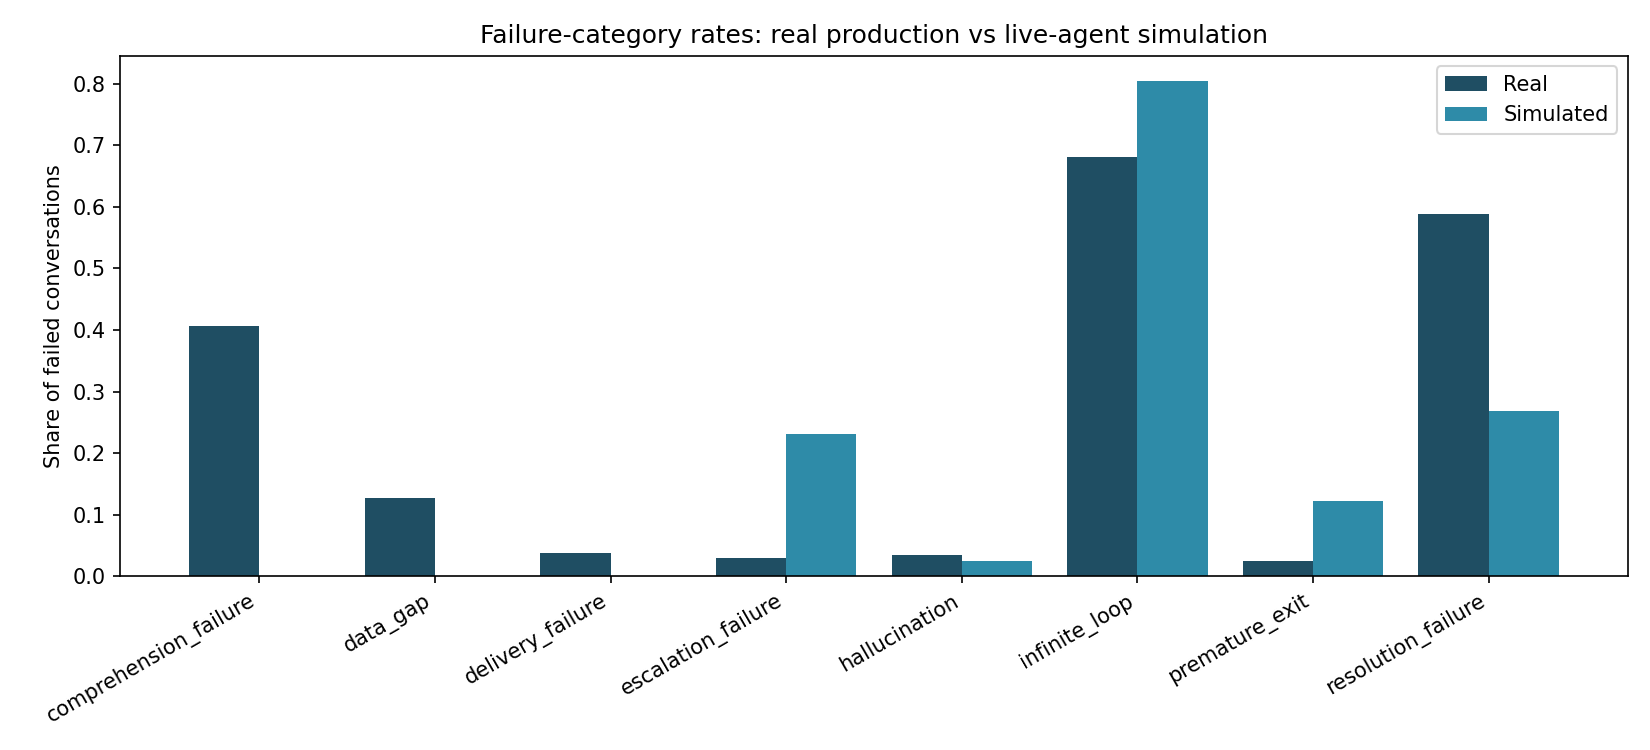
\includegraphics[width=0.95\textwidth]{figures/category_comparison.png}
\caption{Failure-category rates among failed conversations: real production vs live-agent
simulation, identical scorer, shared taxonomy.}
\label{fig:categories}
\end{figure}

\subsection{Distributional divergence}
On the reachable support, $\mathrm{JSD}(\text{real},\text{sim}) = \mathbf{0.2392}$ bits
(95\% CI $[0.2010,\,0.2979]$) --- roughly $48\times$ the split-half sampling noise floor of the
real corpus ($0.0050$), and comparable to the real-vs-uniform anchor ($0.2014$). The honest
reading: at the level of \emph{which} failures occur, correspondence is strong (5/7, matching
dominant mode); at the level of the full \emph{distribution}, the two zero categories dominate
the divergence and keep it far above noise. Including the unreachable category changes little
(JSD $= 0.2470$).

\subsection{Case-level correspondence}
Frequency matching can be coincidental; mechanism matching is stronger evidence. The clearest
matched pair observed: in a simulated test in which the customer disputes information on file,
the agent repeated the \emph{same} phone-number deflection message verbatim for 18 consecutive
turns until the persona abandoned --- a live reproduction of the mechanism behind production's
second-largest failure signal (\cat{loop\_stall}, 256 real failures), where the agent cycles
rather than progresses when it has no path for the customer's actual need. All three simulated
hard failures in the 200-conversation run were of this mechanism.

\section{Results: the scale study}
\label{sec:scale}

Table~\ref{tab:scale} and Figure~\ref{fig:scale} present the seven independent batches and the
cumulative pool.

\begin{table}[H]
\centering
\caption{Scale study: independent batches (top) and cumulative pooling (bottom).
``conv-min'' is summed conversation time; wall time $\approx$ conv-min\,/\,6 workers.}
\label{tab:scale}
\begin{tabular}{rrrrrlrr}
\toprule
$N$ & Failures & Fail rate & Cats & Coverage & JSD vs real (95\% CI) & conv-min & Persona \$ \\
\midrule
10   &   3 & 30.0\% & 2 & 29\% & 0.213 (0.180--0.502) &   3 & 0.05 \\
50   &  12 & 24.0\% & 5 & 71\% & 0.254 (0.192--0.452) &  10 & 0.28 \\
100  &  24 & 24.0\% & 5 & 71\% & 0.232 (0.194--0.330) &  22 & 0.64 \\
200  &  43 & 21.5\% & 4 & 57\% & 0.247 (0.207--0.319) &  38 & 0.96 \\
400  &  90 & 22.5\% & 5 & 71\% & 0.248 (0.213--0.293) &  87 & 2.40 \\
800  & 219 & 27.4\% & 5 & 71\% & 0.225 (0.201--0.259) & 173 & 5.04 \\
1000 & 232 & 23.2\% & 5 & 71\% & 0.242 (0.217--0.276) & 225 & 6.47 \\
\midrule
\multicolumn{8}{c}{\emph{Cumulative pooled}}\\
\midrule
60    &  15 & --- & 5 & 71\% & 0.210 & & \\
360   &  82 & --- & 5 & 71\% & 0.225 & & \\
1560  & 391 & --- & 5 & 71\% & 0.230 & & \\
2560  & 623 & --- & 5 & 71\% & 0.233 & & \\
\bottomrule
\end{tabular}
\end{table}

\begin{figure}[H]
\centering
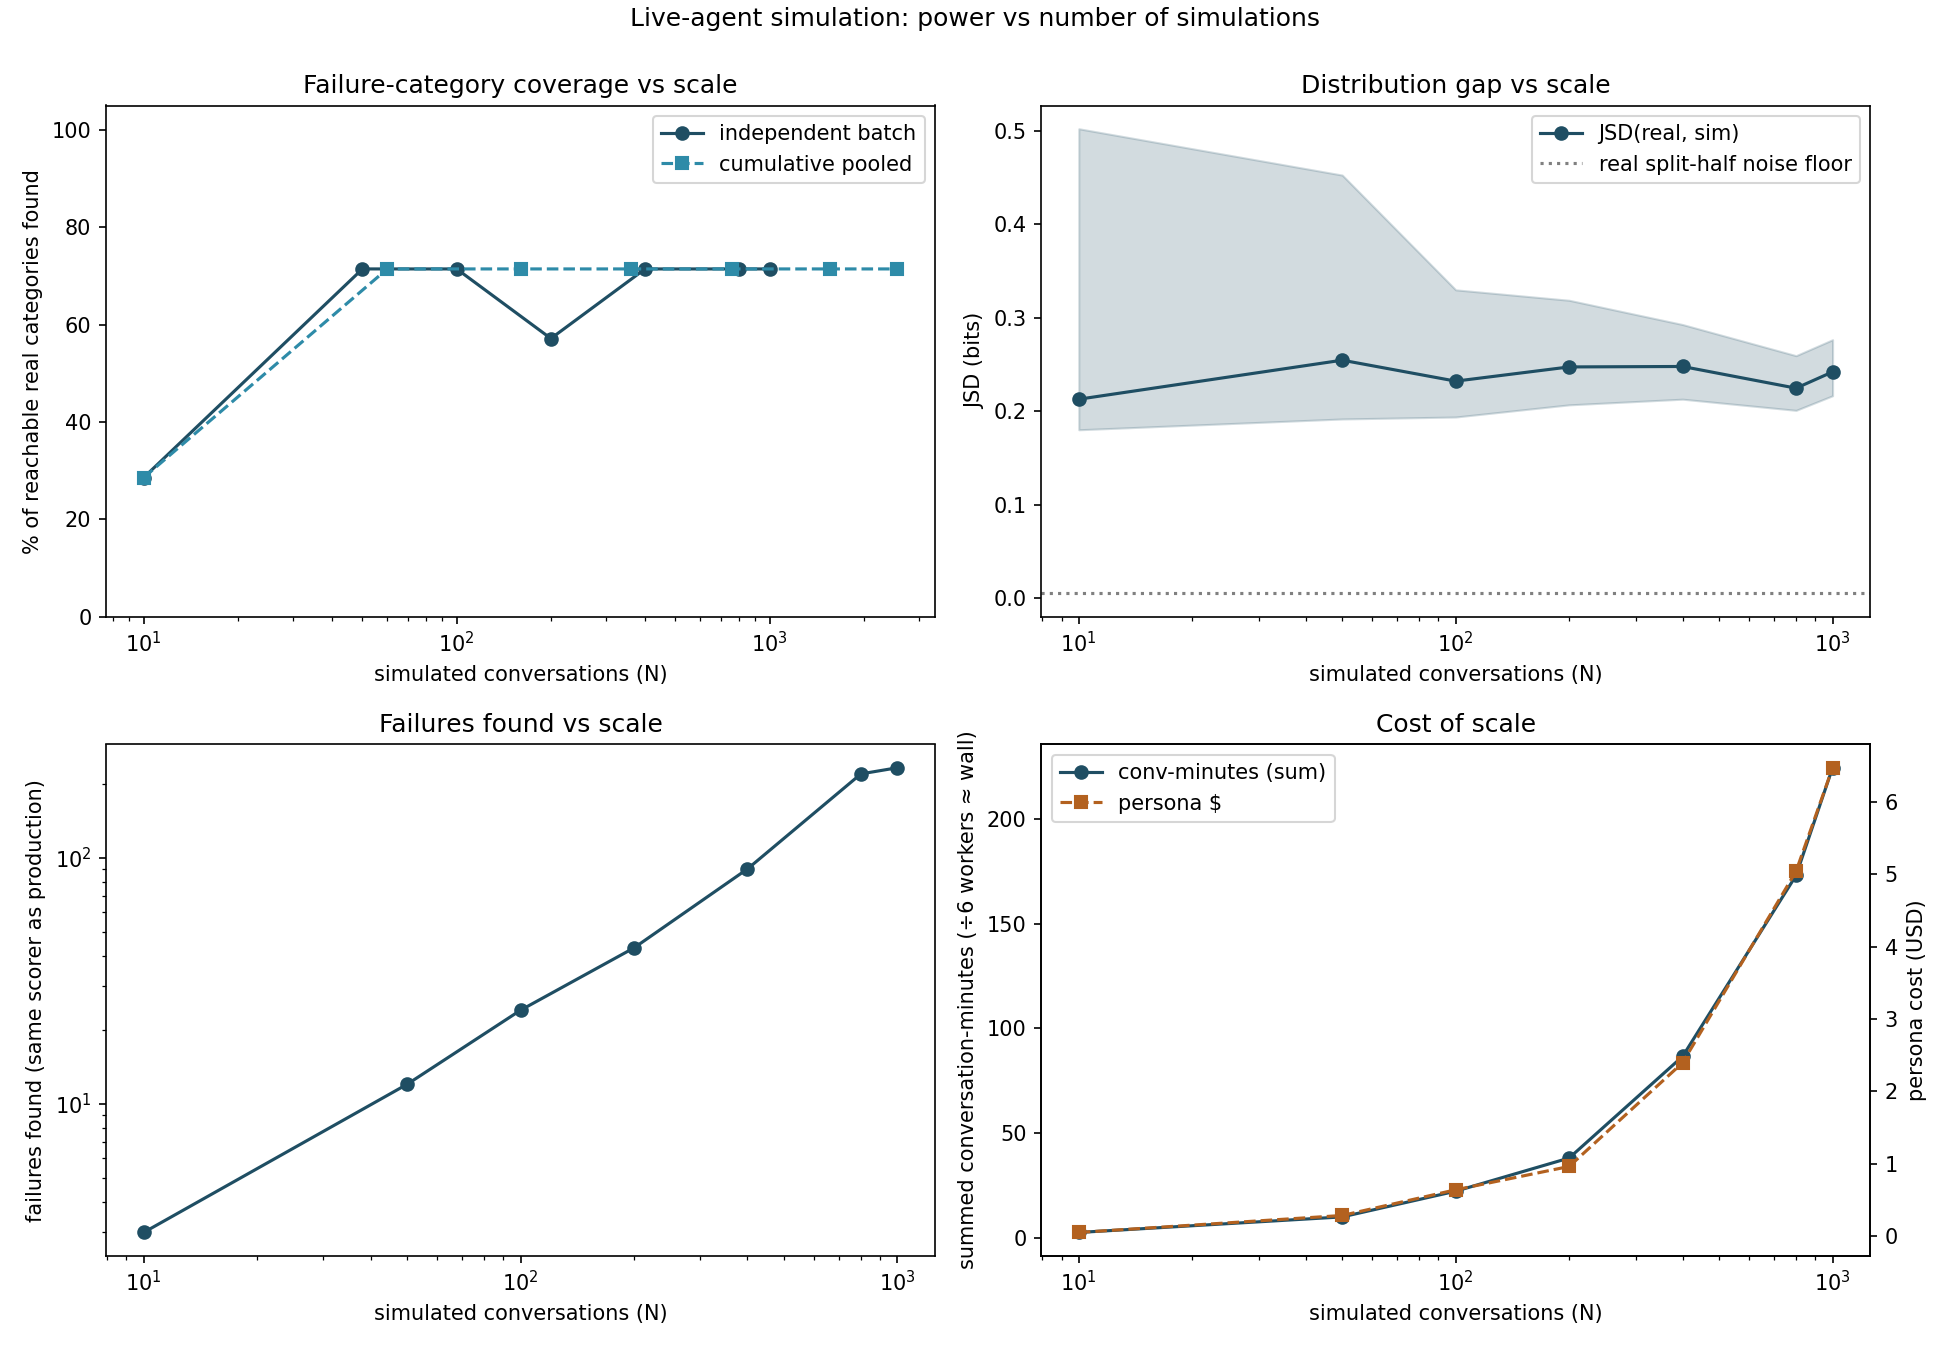
\includegraphics[width=\textwidth]{figures/scale_curves.png}
\caption{Simulation power vs number of simulations (log-$x$). Top-left: category coverage
saturates at $N\!\approx\!50$ (independent and cumulative). Top-right: JSD to the real
distribution is scale-invariant; confidence intervals tighten with $N$. Bottom-left: failures
found grow linearly. Bottom-right: cost of scale.}
\label{fig:scale}
\end{figure}

\noindent Three findings:

\begin{enumerate}[itemsep=2pt]
\item \textbf{Coverage saturates at $N\!\approx\!50$.} A batch of ten finds 2 categories (29\%);
      a batch of fifty finds 5 (71\%); one thousand finds the same 5. The cumulative pool of
      2{,}560 conversations --- $50\times$ the saturation point --- still finds exactly 5.
      (The $N{=}200$ batch's dip to 4 is sampling variance in the rare \cat{hallucination}
      category, whose per-conversation probability is $\sim$1\%.)
\item \textbf{Divergence is scale-invariant; precision is not.} The JSD point estimate stays in
      $[0.21,\,0.25]$ at every scale, while its CI narrows from $\pm0.16$ ($N{=}10$) to
      $\pm0.03$ ($N{=}1000$). Scale buys certainty about the gap, not a smaller gap.
\item \textbf{Failure volume is linear and cheap.} Failures grow proportionally (3 at $N{=}10$;
      232 at $N{=}1000$) at a stable 21--30\% rate; full coverage costs roughly two wall-clock
      minutes and \$0.28 of persona traffic ($N{=}50$); a thousand-conversation batch costs
      $\approx$38 wall-minutes and \$6.47.
\end{enumerate}

\section{Discussion}
\label{sec:discussion}

\paragraph{Simulation power is gated by design, not scale.}
The saturation curve is the report's core message. Everything the simulator \emph{can} find, it
finds almost immediately; what it cannot find at $N{=}50$ it still cannot find at $N{=}2{,}560$.
The two absent categories jointly appear in over half of real failures, so closing them is the
highest-leverage improvement available --- and neither closes by running more simulations.

\paragraph{Why comprehension failures never appear.}
The scorer's reachable comprehension signal is verbatim customer self-repetition. Real customers
repeat themselves --- 376 real conversations contain verbatim repeats --- because they are
frustrated, ignored, or misunderstood. LLM personas rephrase; across all 2{,}950 simulated
conversations, not one repeated itself verbatim twice. This is the over-cooperativity
phenomenon reported in the user-simulation literature, here confirmed on production data with a
pre-registered prediction. The remedy is persona design (explicit repetition/frustration
behaviours), not sampling temperature: published ablations show temperature moves surface
diversity, not behavioural fidelity.

\paragraph{Why data-gap failures never appear.}
The fake customer was built to be \emph{complete} --- every order, warranty state, and CRM row
present --- because the simulation's original purpose was to exercise agent logic. Real backends
are incomplete (missing GSPN rows, stale statuses: 48 real failures). A test database that is
too perfect makes an entire failure class invisible. The remedy is seeding \emph{imperfect}
fixtures: missing orders, null warranty fields, contradictory statuses.

\paragraph{What the simulation over-produces.}
\cat{escalation\_failure} (frustration without hand-off) and \cat{premature\_exit} are
over-represented relative to production. Both excesses trace to adversarial suite composition:
the generated tests deliberately probe refusal and abandonment boundaries that real traffic
rarely exercises. This is the designed purpose of adversarial testing --- finding failures
production has not yet surfaced --- but it means simulated failure \emph{frequencies} should not
be read as production forecasts without reweighting.

\paragraph{Implications.}
For practitioners: a small live-agent simulation ($N\!\approx\!50$, minutes, cents) delivers the
full coverage the current simulator design supports; invest additional budget in simulator
realism, not repetition. For the dissertation: the behavioural result sharpens the static-mode
RQ1 finding --- even with the real agent in the loop, synthetic testing sees a strict subset of
production failure kinds, and the boundary of that subset is now characterised mechanistically.

\section{Threats to validity}
\label{sec:threats}

\begin{enumerate}[itemsep=2pt]
\item \textbf{Rule-based ground truth.} Failure labels come from structured signals; the human
      agreement pass (Cohen's $\kappa$ on a 50-conversation blind packet) is prepared but not yet
      completed. An LLM pilot (lenient agreement 0.86, $\kappa$ 0.51) suggests the criterion
      captures ``customer-unserved friction'' rather than only catastrophic failure. Headline
      claims should be finalised after the human pass.
\item \textbf{Oracle independence.} The comparison deliberately ignores the platform's
      tool-signature test oracles (which mark 94--100\% of these simulated conversations as
      ``passed''); prior work in this project demonstrated such oracles miss semantic failures.
      Scorer parity avoids that bias but inherits the scorer's blind spots symmetrically.
\item \textbf{Suite scope.} All batches draw from one 150-test generated suite (with seeded
      resampling above 150). Saturation at 5 categories is therefore a joint property of
      simulator \emph{and} suite; a differently generated suite (e.g.\ production-feedback-seeded)
      could shift the plateau --- this is the planned arm$\times$context experiment.
\item \textbf{Single seeded customer.} The fake database bounds reachable data-gap and
      multi-customer failure space (pre-registered; observed).
\item \textbf{Clean transport.} Simulated tool calls never time out or rate-limit; chaos
      injection covers only part of this gap, and WhatsApp delivery failure is structurally
      absent (pre-registered as unreachable).
\item \textbf{Anonymisation noise.} Entity scrubbing may weaken fine-grained text signals on the
      real side (repetition detection is exact-match after normalisation and is robust to it).
\end{enumerate}

\section{Conclusion and future work}

Against a verbatim copy of a production agent, LLM-persona simulation reproduces the majority
(5/7) of reachable real failure categories --- including the dominant loop/stall mode with a
mechanistically identical case --- at a production-like failure rate, and does so within
$\sim$50 conversations. What it misses, it misses structurally: over-cooperative personas never
produce comprehension-failure signals, and a too-perfect test database never produces data-gap
failures; 2{,}560 conversations do not buy either back. The distributional gap
(JSD $\approx 0.24$ vs a $0.005$ noise floor) is therefore a design measurement, not a sampling
artefact.

\paragraph{Future work, in leverage order.}
(1)~\emph{Frustrated/repetitive personas}: add explicit repetition and frustration behaviours to
persona generation, then re-measure --- predicted to open \cat{comprehension} and grow
\cat{missed\_escalation} realism. (2)~\emph{Imperfect data seeding}: fixture variants with
missing/contradictory backend rows --- predicted to open \cat{data\_gap}.
(3)~\emph{Arm$\times$context $2\times2$}: blind vs production-feedback-seeded suites, with and
without customer context, $N{=}200$ each --- ties this behavioural analysis to the dissertation's
RQ3/RQ4 feedback result. (4)~\emph{Human annotation pass} to finalise ground-truth validity.
(5)~\emph{Semantic oracles} (X1/X2): the same simulated corpora already contain semantic failures
invisible to both the tool-signature oracles and the rule-based scorer (e.g.\ partially successful
impersonation probes); LLM-judged categories, validated MAST-style against a human-annotated
subsample, would extend the comparison beyond process signals.

\begin{thebibliography}{9}\small

\bibitem{lost} \emph{Lost in Simulation: LLM-Simulated Users are Unreliable Proxies for Human
Users in Agentic Evaluations}, arXiv:2601.17087, 2026.

\bibitem{synthusers} \emph{Synthetic Users, Real Differences: an Evaluation Framework for User
Simulation in Multi-Turn Conversations}, arXiv:2605.02624, 2026.

\bibitem{realusersim} \emph{RealUserSim: Bridging the Reality Gap in Agent Benchmarking via
Grounded User Simulation}, arXiv:2605.20204, 2026.

\bibitem{sim2real} \emph{Mind the Sim2Real Gap in User Simulation for Agentic Tasks},
arXiv:2603.11245, 2026.

\bibitem{mdp} \emph{The Sim-to-Real Gap of Foundation Model Agents: A Unified MDP Perspective},
arXiv:2606.07017, 2026.

\bibitem{mast} M.~Cemri, M.~Z.~Pan, S.~Yang, et al., \emph{Why Do Multi-Agent LLM Systems Fail?},
arXiv:2503.13657, 2025.

\bibitem{gptclick} \emph{What Would GPT Click: Practical Effects of Human-AI Behavioral
Misalignment and the Cost of Synthetic Participants in User Experience}, arXiv:2605.18302, 2026.

\bibitem{jsdpower} \emph{Statistical Properties and Power Analysis of Divergence Measures for
Credit Risk Model Monitoring}, arXiv:2607.12407, 2026.

\bibitem{latitude} \emph{Why AI Agents Break in Production: Failure Patterns and How to Detect
Them}, Latitude Engineering Blog, 2026.

\end{thebibliography}

\appendix
\section{Reproducibility}
All artefacts live in the \texttt{investigation/} package accompanying this report:
the anonymised real corpus (\texttt{02\_data/real/}), every simulated corpus as consolidated
\texttt{conversations.json} exports (\texttt{02\_data/simulated/}, including the seven scale
batches with run reports and failure inboxes), the three analysis scripts
(\texttt{03\_analysis\_scripts/}), and machine-readable results
(\texttt{04\_results/}). The comparison regenerates with:
\begin{quote}\ttfamily\small
python3 compare\_real\_vs\_sim.py --real tech_repair-conversations-anonymized.json \textbackslash\\
\hspace*{1.5em} --sim <conversations.json> [--sim \ldots] -o <outdir>\\
python3 scale\_curves.py --real tech_repair-conversations-anonymized.json \textbackslash\\
\hspace*{1.5em} --batches results\_scale\_study -o <outdir>
\end{quote}
Scale-study suites regenerate byte-identically from seeds ($42{+}N$) via
\texttt{gen\_scale\_suites.py}. The raw (non-anonymised) export is deliberately excluded from
this package.

\end{document}
